\documentclass[xcolor=pdflatex,dvipsnames,table]{beamer}
\usepackage{epsfig,graphicx}
\usepackage{palatino}
\usepackage{fancybox}
\usepackage{relsize}
\usepackage[procnames]{listings}
\usepackage{hyperref}
\usepackage{qtree} % needed?
\usepackage{booktabs}
\usepackage{dirtree}
\usepackage[normalem]{ulem}


% fatter TT font
\renewcommand*\ttdefault{txtt}
% another TT, suggested by Alex
% \usepackage{inconsolata}
% \usepackage[T1]{fontenc} % needed as well?


\newcommand{\scale}{0.7}

\newcommand{\todo}[1]{{\emph{TODO: #1}}}
\newcommand{\martin}[1]{{\color{blue} Martin: #1}}
\newcommand{\abcdef}[1]{{\color{red} Author2: #1}}

% uncomment following for final submission
%\renewcommand{\todo}[1]{}
%\renewcommand{\martin}[1]{}
%\renewcommand{\author2}[1]{}

\newcommand{\code}[1]{{\texttt{#1}}}

\hypersetup{
  linkcolor  = black,
%  citecolor  = blue,
  urlcolor   = blue,
  colorlinks = true,
}

\beamertemplatenavigationsymbolsempty
\setbeamertemplate{footline}[frame number]





\newif\ifbook
% shared in slides and book

\lstdefinelanguage{chisel}{
%  morekeywords={abstract,case,catch,class,def,%
%    do,else,extends,false,final,finally,%
%    for,if,implicit,import,match,mixin,%
%    new,null,object,override,package,%
%    private,protected,requires,return,sealed,%
%    super,this,throw,trait,true,try,%
%    type,val,var,while,with,yield},
%  otherkeywords={=>,<-,<\%,<:,>:,\#,@},
  sensitive=true,
  morecomment=[l]{//},
  morecomment=[n]{/*}{*/},
  morestring=[b]",
  morestring=[b]',
  morestring=[b]"""
}

\usepackage{color}
\definecolor{dkgreen}{rgb}{0,0.6,0}
\definecolor{gray}{rgb}{0.5,0.5,0.5}
\definecolor{mauve}{rgb}{0.58,0,0.82}

% Default settings for code listings
%\ifbook
\lstset{%frame=lines,
  language=chisel,
  aboveskip=3mm,
  belowskip=3mm,
  showstringspaces=false,
  columns=fixed, % basewidth=\mybasewidth,
  basicstyle={\small\ttfamily},
  numbers=none,
  numberstyle=\footnotesize,
  % identifierstyle=\color{red},
  breaklines=true,
  breakatwhitespace=true,
  procnamekeys={def, val, var, class, trait, object, extends},
  % procnamestyle=\ttfamily,
  tabsize=2,
  float
}
%\else
%\lstset{%frame=lines,
%  language=chisel,
%  aboveskip=3mm,
%  belowskip=3mm,
%  showstringspaces=false,
%  columns=fixed, % basewidth=\mybasewidth,
%  basicstyle={\small\ttfamily},
%  numbers=none,
%  numberstyle=\footnotesize\color{gray},
%  % identifierstyle=\color{red},
%  keywordstyle=\color{blue},
%  commentstyle=\color{dkgreen},
%  stringstyle=\color{mauve},
%  breaklines=true,
%  breakatwhitespace=true,
%  procnamekeys={def, val, var, class, trait, object, extends},
%  procnamestyle=\ttfamily\color{red},
%  tabsize=2,
%  float
%}
%\fi

\lstnewenvironment{chisel}[1][]
{\lstset{language=chisel,#1}}
{}

\newcommand{\shortlist}[1]{{\lstinputlisting[nolol]{#1}}}

\newcommand{\longlist}[3]{{\lstinputlisting[float, caption={#2}, label={#3}, frame=tb, captionpos=b]{#1}}}

\newcommand{\verylonglist}[3]{{\lstinputlisting[caption={#2}, label={#3}, frame=tb, captionpos=b]{#1}}}


\title{Interfacing and Memory}
\author{Martin Schoeberl}
\date{\today}
\institute{Technical University of Denmark\\
Embedded Systems Engineering}

\begin{document}

\begin{frame}
\titlepage
\end{frame}


\begin{frame}[fragile]{Overview}
\begin{itemize}
\item Repeat FSMD (for the vending machine)
\begin{itemize}
\item I have seen some intermix of FSM and datapath
\item Works only for small designs
\end{itemize}
\item Interfaces
\item Memory (intern and extern)
\item Serial interface (RS 232)
\item Testing with Chisel (repetition)
\item 2 hours testing exerise
\item The course evaluation is open for feedback
\begin{itemize}
\item Closes 1st May night
\end{itemize}
\item Next week we will do a test exam
\end{itemize}
\end{frame}

\begin{frame}[fragile]{I have seen similar code}
\begin{chisel}
  when(io.coin2) {
    sum := sum + 2.U
  } .elsewhen(io.coin5) {
    sum := sum + 5.U
  }
\end{chisel}
\begin{itemize}
\item This may work for tiny projects
\item This style does not scale for larger designs
\item I recommend using an FSM + datapath
\begin{itemize}
\item Split responsibility
\item Can be individually tested
\item Can be developed in parallel
\end{itemize}
\end{itemize}
\end{frame}


\begin{frame}[fragile]{Using an FSM and a Datapath}
\begin{itemize}
\item About the design of the vending machine (VM)
\item Some of you start coding the VM directly
\begin{itemize}
\item This may work for small designs
\item But does not scale
\end{itemize}
\item Better use a systematic approach
\item Use a FSM that communicates with a datapath (FSMD)
\item We will quickly repeat FSMD
\end{itemize}
\end{frame}



\begin{frame}[fragile]{Finite-State Machine (FSM)}
\begin{itemize}
\item Has a register that contains the state
\item Has a function to computer the next state
\begin{itemize}
\item Depending on current state and input
\end{itemize}
\item Has an output depending on the state
\item Use a Moore FSM for the VM
\end{itemize}
\end{frame}

\begin{frame}[fragile]{Basic Finite-State Machine}
\begin{itemize}
\item A state register
\item Two combinational blocks
\end{itemize}
\begin{figure}
  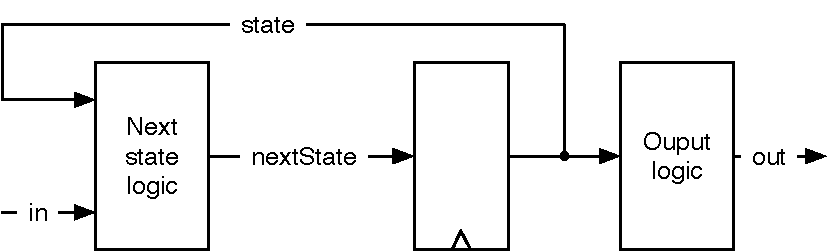
\includegraphics[scale=\scale]{../figures/fsm}
\end{figure}
\end{frame}

\begin{frame}[fragile]{State Diagram}
\begin{figure}
  \includegraphics[scale=\scale]{../figures/state-diag-moore}
\end{figure}
\begin{itemize}
\item States and transitions depending on input values
\item Example is a simple alarm FSM
\item Nice visualization
\item Draw the state diagram for your VM during the design
\item Include a state diagram in the report
\end{itemize}
\end{frame}


\begin{frame}[fragile]{Encoding the State}
\begin{itemize}
\item We can optimize state encoding
\item Two common encodings are: binary and one-hot
\item We leave it to the synthesize tool
\item Use symbolic names with an \code{Enum}
\item Note the number of states in the \code{Enum} construct
\item We use a Scala list with the \code{::} operator
\end{itemize}
\shortlist{../code/simple_fsm_states.txt}
\end{frame}

\begin{frame}[fragile]{Start the FSM}
\begin{itemize}
\item We have a starting state on reset
\end{itemize}
\shortlist{../code/simple_fsm_register.txt}
\end{frame}


\begin{frame}[fragile]{The Next State Logic}
\shortlist{../code/simple_fsm_next.txt}
\end{frame}


\begin{frame}[fragile]{FSM with Datapath}
\begin{itemize}
\item A type of computing machine
\item Consists of a finite-state machine (FSM) and a datapath
\item The FSM is the master (the controller) of the datapath
\item The datapath has computing elements
\begin{itemize}
\item E.g., adder, incrementer, constants, multiplexers, ...
\end{itemize}
\item The datapath has storage elements (registers)
\begin{itemize}
\item E.g., sum of money payed, count of something, ...
\end{itemize}
\item You VM design shall be a FSMD
\end{itemize}
\end{frame}

\begin{frame}[fragile]{FSM-Datapath Interaction}
\begin{itemize}
\item The FSM controls the datapath
\begin{itemize}
\item For example, add 2 to the sum
\end{itemize}
\item By controlling multiplexers
\begin{itemize}
\item For example, select how much to add
\item Not adding means selecting 0 to add
\end{itemize}
\item Which value goes where
\item The FSM logic also depends on datapath output
\begin{itemize}
\item Is there enough money payed to release a can of soda?
\end{itemize}
\item FSM and datapath interact
\end{itemize}
\end{frame}


\begin{frame}[fragile]{Popcount Example}
\begin{itemize}
\item An FSMD that computes the popcount
\item Also called the Hamming weight
\item Compute the number of `1's in a word
\item Input is the data word
\item Output is the count
\end{itemize}
\end{frame}

\begin{frame}[fragile]{Popcount Block Diagram}

\begin{figure}
  \includegraphics[scale=\scale]{../figures/popcnt-fsmd}
\end{figure}
\end{frame}


\begin{frame}[fragile]{The FSM}
\begin{figure}
  \includegraphics[scale=\scale]{../figures/popcnt-states}
\end{figure}
\begin{itemize}
\item A Very Simple FSM
\item Two transitions depend on input/output handshake
\item One transition on the datapath output
\end{itemize}
\end{frame}

\begin{frame}[fragile]{The Datapath}
\begin{figure}
  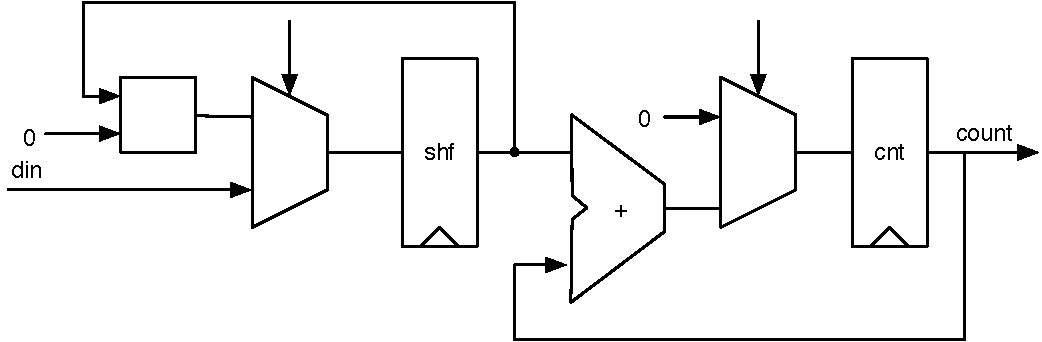
\includegraphics[scale=0.65]{../figures/popcnt-data}
\end{figure}
\end{frame}

\begin{frame}[fragile]{Let's Explore the Code}
\begin{itemize}
\item In \href{https://github.com/schoeberl/chisel-book/blob/master/src/main/scala/PopCount.scala}{PopCount.scala}
\end{itemize}
\end{frame}

\begin{frame}[fragile]{Usage of an FSMD}
\begin{itemize}
\item Of course for your VM
\begin{itemize}
\item The VM is a simple processor
\item But not Turing complete
\item Can \emph{only} process coins of 2 and 5
\end{itemize}
\item Have the FSM and the data path in two \code{Module}s
\item An FSMD can be used to build a processor
\item Fine for simple processors
\item E.g., \href{https://github.com/schoeberl/lipsi}{Lipsi}
\item Pipelined processor topic of
\begin{itemize}
\item Computer Architecture Engineering (02155)
\end{itemize}\end{itemize}
\end{frame}

\begin{frame}[fragile]{Use a FSMD for the VM}
\begin{itemize}
\item This is the main part your vending machine
\item Can be design and tested just with Chisel testers (no FPGA board needed)
\item See the given tester
\begin{itemize}
\item Sets the price to 7
\item Adds two coins (2 and 5)
\item Presses the buy button
\end{itemize}
\item Extend the test along the development
\begin{itemize}

\item Remember test driven development?
\item Maybe write the test before the implementation
\item Maybe test developer and FSMD developer are not always the same person
\end{itemize}
\end{itemize}
\end{frame}

\begin{frame}[fragile]{Code Snippets for the VM}
\begin{chisel}
  val idle :: add2 ... :: Nil = Enum(?)
  val stateReg = RegInit(idle)
  ...
  switch (stateReg) {
    is (idle){
      when(coin2) {
        stateReg := ...
      }
      when(...) {
   ...
   switch(stateReg) {
     is (add2) { ... }  // drive the datapath for adding a coin of kr. 2
\end{chisel}
\end{frame}

\begin{frame}[fragile]{Memory}
\begin{itemize}
\item Registers are storage elements == memory
\item Just use a \code{Reg} of a \code{Vec}
\item This is 1 KiB of memory
\begin{chisel}
  val memoryReg = Reg(Vec(1024, UInt(8.W)))
  // writing into memory
  memoryReg(wrAddr) := wrData
  // reading from the memory
  val rdData = memoryReg(rdAddr)
\end{chisel}
\item Simple, right?
\item But is this a good solution?
\end{itemize}
\end{frame}

\begin{frame}[fragile]{A Flip-Flop}
\begin{itemize}
\item Remember the circuit of a register (flip-flop)?
\item Two latches: \href{https://en.wikipedia.org/wiki/Flip-flop_(electronics)#Master%E2%80%93slave_edge-triggered_D_flip-flop}{master and slave}
\item One (enable) latch can be built with 4 NAND gates
\item a NAND gate needs 6 transistors, an inverter 2 transistors
\item A flip-flop needs 20 transistors (for a single bit)
\item Can we do better?
\end{itemize}
\end{frame}

\begin{frame}[fragile]{A Memory Cell}
\begin{itemize}
\item A single bit can be stored in \href{https://en.wikipedia.org/wiki/Static_random-access_memory#/media/File:SRAM_Cell_(6_Transistors).svg}{6 transistors}
\item That is how larger memories are built
\item FPGAs have this type of on-chip memories
\item Usually many of them in units of 2 KiB or 4 KiB
\item We need some Chisel code to represent it
\item More memory needs an extra chip
\item Then we need to interface this memory from the FPGA
\end{itemize}
\end{frame}

\begin{frame}[fragile]{SRAM Memory}
\begin{itemize}
\item RAM stands for random access memory
\item SRAM stands for static RAM
\item There is also something called DRAM for dynamic RAM
\begin{itemize}
\item Uses a capacitor and a transistor
\item DRAM is smaller than SRAM
\item But needs refreshes
\item Different technology than technology for logic
\end{itemize}
\item All on-chip memory is SRAM (today)
\end{itemize}
\end{frame}

\begin{frame}[fragile]{Memory Interface}
\begin{itemize}
\item Interface
\begin{itemize}
\item Address input (e.g., 10 bits for 1 KiB)
\item Write signal (e.g., we)
\item Data input
\item Data output
\end{itemize}
\item May share pins for the data input and output (tri-state)
\item May have read and write addresses
\begin{itemize}
\item A so-called dual ported memory
\item Can do a read and a write in the same clock cycle
\end{itemize}
\end{itemize}
\end{frame}


\begin{frame}[fragile]{On-Chip Memory}
\begin{itemize}
\item SRAM by itself is asynchronous
\item No clock, just the correct timing
\item Apply the address and after some time the data is valid
\item But one can add input registers, which makes it a synchronous SRAM
\item Current FPGAs have only synchronous memories
\item FPGAs usually have dual-ported memories
\item This means the result of a read is available on clock cycle after the address is given
\begin{itemize}
\item This is different from the use of flip-flops (\code{Reg(Vec(..))})
\end{itemize}
\end{itemize}
\end{frame}

\begin{frame}[fragile]{Synchronous Memory}
\begin{figure}
  \includegraphics[scale=\scale]{../figures/memory}
\end{figure}
\end{frame}

\begin{frame}[fragile]{Use of a Chisel SyncReadMem}
\shortlist{../code/memory.txt}
\end{frame}

\begin{frame}[fragile]{Read-During-Write}
\begin{itemize}
\item What happens when one writes to and reads from the same address?
\item Which value is returned?
\item Three possibilities:
\begin{enumerate}
\item The newly written value
\item The old value
\item Undefined (mix of old and new)
\end{enumerate}
\item Depends on technology, FPGA family, ...
\item We want to have a defined read-during-write
\item We add hardware to \emph{forward} the written value
\end{itemize}
\end{frame}

\begin{frame}[fragile]{Condition for Forwarding}
\begin{itemize}
\item If read and write addresses are equal
\item If write enable is true
\item Multiplex the output to take the new write value instead of the (old) read value
\item Delay that forwarded write value to have the same timing
\end{itemize}
\end{frame}

\begin{frame}[fragile]{Memory with Forwarding}
\begin{figure}
  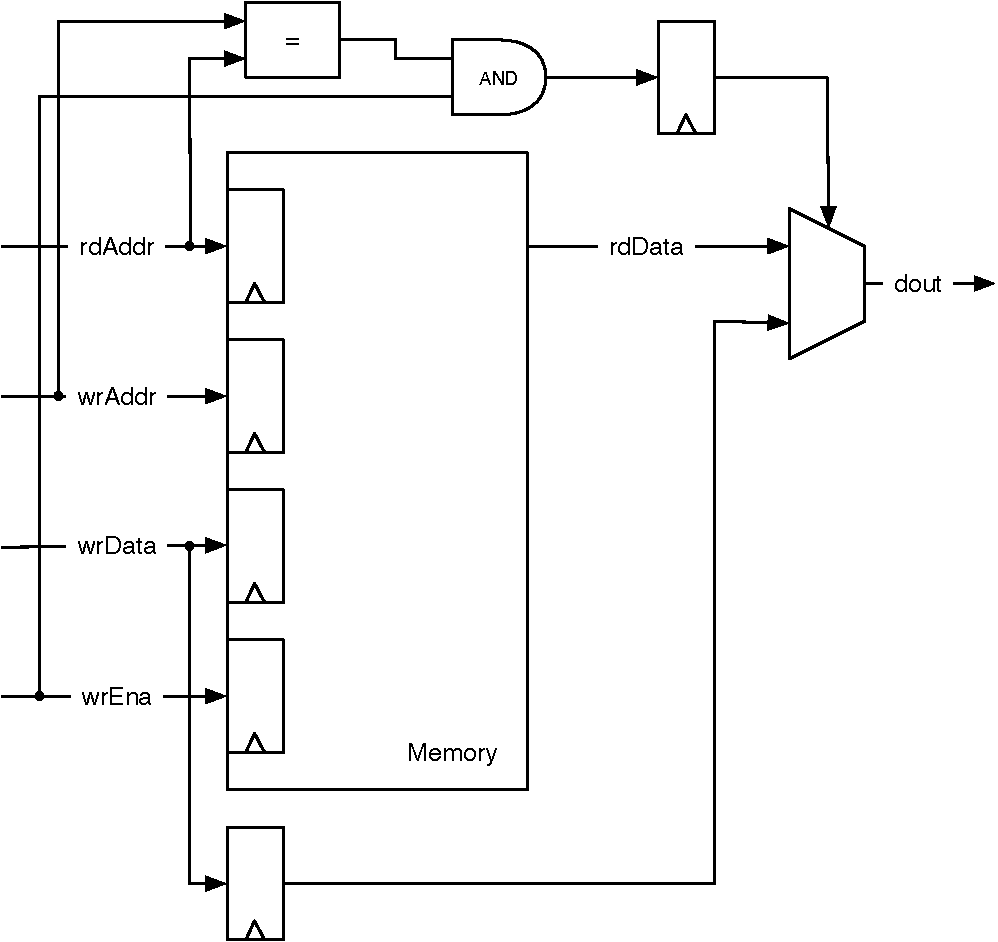
\includegraphics[scale=0.5]{../figures/memory-forwarding}
\end{figure}
\end{frame}

\begin{frame}[fragile]{Forwarding in Chisel}
\begin{chisel}
  val mem = SyncReadMem(1024, UInt(8.W))

  val wrDataReg = RegNext(io.wrData)
  val doForwardReg = RegNext(io.wrAddr === io.rdAddr && io.wrEna)

  val memData = mem.read(io.rdAddr)

  when(io.wrEna) {
    mem.write(io.wrAddr, io.wrData)
  }

  io.rdData := Mux(doForwardReg, wrDataReg, memData)
\end{chisel}
\end{frame}


\begin{frame}[fragile]{External Memory}
\begin{itemize}
\item On-chip memory is limited
\item We can add an external memory chip
\begin{itemize}
\item Is cheaper than FPGA on-chip memory
\end{itemize}
\item Sadly the Basys3 board has no external memory
\item Simple memory is an asynchronous SRAM
\end{itemize}
\end{frame}

\begin{frame}[fragile]{External SRAM}
\begin{itemize}
\item We \emph{buy} a CY7C1041CV33
\item Let us look into the \href{https://cn.inside.dtu.dk/cnnet/filesharing/download/618360ca-01b4-42e4-86e2-765835963deb}{data sheet}
\end{itemize}
\end{frame}

\begin{frame}[fragile]{Interfacing the SRAM}
\begin{itemize}
\item FPGA output drives address, control, and data (sometimes)
\item FPGA reads data
\item The read signal is asynchronous to the FPGA clock
\item Do we need an input synchronizer?
\end{itemize}
\end{frame}

\begin{frame}[fragile]{Synchronous Interface}
\begin{itemize}
\item Logic is synchroous
\item Memory is asynchronous
\begin{itemize}
\item How to interface?
\end{itemize}
\item Output signals
\begin{itemize}
\item Generate timing with synchronous circuit
\item Small FSM
\end{itemize}
\item Asynchronous input signale
\begin{itemize}
\item Usually 2 register for input synchronization
\item Really needed for the SRAM interface?
\item We would loose 2 clock cycles
\end{itemize}
\end{itemize}
\end{frame}


\begin{frame}[fragile]{SRAM Read}
\begin{itemize}
\item Asynchronous timing definition (data sheet)
\item But, we know the timing and we trigger the SRAM address from
our synchronous design
\item No need to use synchronization registers
\item \emph{Just} get the timing correct
\item Draw the example
\begin{itemize}
\item Address - SRAM - data
\item Relative to the FPGA clock
\end{itemize}
\end{itemize}
\end{frame}

\begin{frame}[fragile]{Read Timing Continued}
\begin{itemize}
\item Add all time delays
\begin{itemize}
\item Within FPGA
\item Pad to pin
\item PCB traces
\item SRAM read timing
\item PCB traces back
\item Pin to pad
\item Into FPGA register
\end{itemize}
\item Setup and hold time for FPGA register
%\item Is your today's lab exercise
\end{itemize}
\end{frame}

\begin{frame}[fragile]{Connecting to the World}
\begin{itemize}
\item Logic in the FPGA
\begin{itemize}
\item Described in Chisel
\item Abstracting away electronic properties
\end{itemize}
\item Interface to the world
\begin{itemize}
\item Simple switches and LEDs
\item Did we think about timing?
\end{itemize}
\item FPGA is one component of the system
\item Need interconnect to
\begin{itemize}
\item Write outputs
\item Read inputs
\item Connect to other chips
\end{itemize}
\end{itemize}
\end{frame}

\begin{frame}[fragile]{Bus Interface}
\begin{itemize}
\item Memory interface can be generalized
\item We use a so-called bus to connect several devices
\item Usually a microprocessor connected to devices (memory, IO)
\item The microprocessor is the master
\item A bus is an interface definition
\begin{itemize}
\item Logic and timing
\item Electrical interface
\end{itemize}
\item Parallel or serial data
\item Asynchronous or synchronous
\begin{itemize}
\item But interface clock is usually not the logic clock
\end{itemize}
\end{itemize}
\end{frame}

\begin{frame}[fragile]{Bus Properties}
\begin{itemize}
\item Address bus and data bus
\item Control lines (read and write)
\item Several devices connected
\begin{itemize}
\item Multiple outputs
\item Use tri-state to avoid multiple driver
\end{itemize}
\item Single or multiple master
\begin{itemize}
\item Arbitration for multiple master
\end{itemize}
\item Sketch a small microprocessor system
\end{itemize}
\end{frame}

\begin{frame}[fragile]{Serial I/O Interface}
\begin{itemize}
\item Use only one wire for data transfer
\begin{itemize}
\item Bits are serialized
\item That is where you need your shift register
\end{itemize}
\item Shared wire or dedicated wires for transmit and receive
\item Self timed
\begin{itemize}
\item Serial UART (RS 232)
\item Ethernet
\item USB
\end{itemize}
\item With a clock signal
\begin{itemize}
\item SPI, I2C, ...
\end{itemize}
\end{itemize}
\end{frame}



\begin{frame}[fragile]{RS 232}
\begin{itemize}
\item Old, but still common interface standard
\begin{itemize}
\item Was common in 90' in PCs
\item Now substituted by USB
\item Still common in embedded systems
\item Your Basys3 board has a RS 232 interface
\end{itemize}
\item Standard defines
\begin{itemize}
\item Electrical characteristics
\item '1' is negative voltage (-15 to -3 V)
\item '0' is positive voltage (+3 to +15 V)
\item Converted by a RS 232 driver to \emph{normal} logic voltage levels
\end{itemize}
\end{itemize}
\end{frame}


\begin{frame}[fragile]{Serial Transmission}
\begin{itemize}
\item Transmission consists of
\begin{itemize}
\item Start bit
\item 8 data bits
\item Stop bit(s)
\end{itemize}
\item Common baud rate is 115200 bits/s
\end{itemize}
\begin{figure}
  \includegraphics[scale=0.8]{../figures/uart_wave}
\end{figure}
\end{frame}


\begin{frame}[fragile]{RS 232 Interface}
\begin{itemize}
\item Generate bit clock with with counter
\begin{itemize}
\item Like clock tick generation for display multiplexer
\end{itemize}
\item Output (transmit)
\begin{itemize}
\item Use shift register for parallel to serial conversion
\item Small FSM to generate start bit, data bits, and stop bits
\end{itemize}
\item Input (receive)
\begin{itemize}
\item Detect start with the falling edge of the start bit
\item \emph{Position} into middle of start bit
\item Sample individual bits
\item Serial to parallel conversion with a shift register
\end{itemize}
\end{itemize}
\end{frame}


\begin{frame}[fragile]{Chisel Code for RS 232}
\begin{itemize}
\item More explanation can be found in section 11.2
\item The code is in the Chisel book
\item \href{https://github.com/schoeberl/chisel-book/blob/master/src/main/scala/uart.scala}{uart.scala}
\item Also see example usage in \href{https://github.com/schoeberl/chisel-examples}{chisel-examples} repo
\end{itemize}
\end{frame}

\begin{frame}[fragile]{RS 232 on the Basys3}
\begin{itemize}
\item Basys3 has an FTDI chip for the USB interface
\item USB interface for FPAG programming
\item But also to provide a RS 232 to the FPGA
\item You can talk with your laptop
\item Your VM could write out some text
\item Use the Chisel code I showed you
\item Open a terminal to watch % (show it)
\end{itemize}
\end{frame}

\begin{frame}[fragile]{RS 232 from ip-contributions}
\begin{itemize}
\item A collection of Chisel hardware components
\item Contains the RS232 interface
\item Distributed as library from Maven Central
\item No need to copy source around
\item Just include it in your \code{build.sbt}
\item Very easy distribution of open-source components
\item You can contribute!
\item \href{https://github.com/freechipsproject/ip-contributions}{ip-contributions}
\end{itemize}
\end{frame}

\begin{frame}[fragile]{Testing and Debugging}
\begin{itemize}
\item For debugging waveforms are fine
\item Can become cumbersome as it needs \emph{manual inspection}
\item Better having real tests
\item Tests that check the result
\item Can also be automated (e.g, continuous integration)
\item Writing testers in Chisel may include some Scala code
\item In principle you could also include Java code for testing ;-)
\end{itemize}
\end{frame}

\begin{frame}[fragile]{Testing with Chisel}
\begin{itemize}
\item Set input values with \code{poke}
\item Advance the simulation with \code{step}
\item Read the output values with \code{peek}
\item Compare the values with \code{expect}
\item Import following packages:
\shortlist{../code/test_import.txt}
\end{itemize}
\end{frame}

\begin{frame}[fragile]{A Chisel Tester}
\begin{itemize}
\item Extends class \code{PeekPokeTester}
\item Has the device-under test (DUT) as parameter
\item Testing code can use all features of Scala
\end{itemize}
\begin{chisel}
class CounterTester(dut: Counter) extends PeekPokeTester(dut) {

  // Here comes the Chisel/Scala code
  // for the testing
}
\end{chisel}
\end{frame}

\begin{frame}[fragile]{Example DUT}
\begin{itemize}
\item A device-under test (DUT)
\shortlist{../code/test_dut.txt}
\end{itemize}
\end{frame}


\begin{frame}[fragile]{The Main Program for the Test}
\begin{itemize}
\item Extend an App and invoke the \code{iotesters} driver
\item With the DUT and the tester
\shortlist{../code/test_main_simple.txt}
\end{itemize}
\end{frame}

\begin{frame}[fragile]{A Tester}
\begin{itemize}
\item Poke values and \code{expect} some output
\shortlist{../code/test_bench.txt}
\end{itemize}
\end{frame}

\begin{frame}[fragile]{ScalaTest}
\begin{itemize}
\item Testing framework for Scala
\item Tests live in \code{src/test/scala}
\item \code{sbt} understands ScalaTest
\item Run all tests:
\code{sbt test}
\item When all \code{expect}s are ok, the test passes
\item A little bit funny syntax
\item Add library to \code{build.sbt}
\begin{chisel}
libraryDependencies += "org.scalatest" %% "scalatest" % "3.0.5" % "test"
\end{chisel}
\item Import ScalaTest library
\begin{chisel}
import org.scalatest._
\end{chisel}
\end{itemize}
\end{frame}

\begin{frame}[fragile]{ScalaTest Version of our Tester}
\shortlist{../code/scalatest_simple.txt}
\end{frame}

\begin{frame}[fragile]{Testing Your Vending Machine}
\begin{itemize}
\item Write (unit) tests for each component/module
\item E.g., one for the data path, one for the state machine
\item Then one (integration) test for the top-level component/module
\item Maybe do some \href{https://en.wikipedia.org/wiki/Extreme_programming}{extreme programming (XP)}
\begin{itemize}
\item Write the test first
\item Then the code of the component
\item The test can serve as a specification
\item We can do \href{https://en.wikipedia.org/wiki/Agile_software_development}{agile} hardware development
\end{itemize}
\end{itemize}
\end{frame}

\begin{frame}[fragile]{Today's Lab}
\begin{itemize}
\item You requested a testing exercise at the midterm evaluation
\item Testing a 5:1 Mux that contains errors
\item see \href{https://github.com/schoeberl/chisel-lab/tree/master/lab11}{lab 11}
\item As usual, show and discuss with a TA
\end{itemize}
\end{frame}


%\begin{frame}[fragile]{Today's Lab}
%\begin{itemize}
%\item Paper \& pencil exercises on SRAM interfacing
%\item On paper or in a plain text editor
%\item As usual, show and discuss with a TA
%\item Exercise description is in DTU Inside file sharing
%\item \href{https://cn.inside.dtu.dk/cnnet/filesharing/download/39a98e6a-f453-4aa7-98c4-cb13eae6c805}{sram\_exercise.pdf}
%\item \href{https://cn.inside.dtu.dk/cnnet/filesharing/download/618360ca-01b4-42e4-86e2-765835963deb}{SRAM data sheet: CYCC1041...}
%\end{itemize}
%\end{frame}

\begin{frame}[fragile]{Summary}
\begin{itemize}
\item Use an FSMD for the vending machine and simple processors
\item We need to connect to the world
\item FPGA (or any chip) is only part of a system
\item Bus interface to external devices (e.g., memory)
\item Serial interface to connect systems
\begin{itemize}
\item E.g., your Basys3 board to the laptop
\end{itemize}
\item Testing is more than looking at waveforms
\end{itemize}
\end{frame}



\end{document}

%\begin{frame}[fragile]{xxx}
%\begin{itemize}
%\item yyy
%\end{itemize}
%\end{frame}
